%%%%%%%%%%%%%%%%%%%%%%%%%%%%%%%%%%%%%%%%%%%%%%%%%%%%%%%%%%%%%%%%%%%%%%%
%%%%  Load the document class and packages                         %%%%
%%%%%%%%%%%%%%%%%%%%%%%%%%%%%%%%%%%%%%%%%%%%%%%%%%%%%%%%%%%%%%%%%%%%%%%
\documentclass[a4paper]{report}
\usepackage{epsfig}            % to insert PostScript figures
\graphicspath{ 
  {./figures} 
}

%Change figure names
\renewcommand{\figurename}{Fig}

\usepackage[bf,footnotesize]{caption} % make captions small and label bold


\addtocounter{chapter}{1} %Because starting at zero is silly
\makeatletter
\renewcommand{\thesection}{\@arabic\c@section}
\renewcommand{\thefigure}{\@arabic\c@figure}
\makeatother

\usepackage[a4paper,margin=2.7cm,tmargin=2.5cm,bmargin=2.5cm]{geometry} 
\usepackage{textcomp}          % To make nice degree symbols and others\usepackage[bf,footnotesize]{caption} % make captions small and label bold
\usepackage{wrapfig}
%to produce the clickable references along the left in Acroread. This
%package must be included last. 
\usepackage[ps2pdf,bookmarks=TRUE]{hyperref} 



%%%%%%%%%%%%%%%%%%%%%%%%%%%%%%%%%%%%%%%%%%%%%%%%%%%%%%%%%%%%%%%%%%%%%%%
%%%%  Hypertext references for Acrobat                             %%%%
%%%%%%%%%%%%%%%%%%%%%%%%%%%%%%%%%%%%%%%%%%%%%%%%%%%%%%%%%%%%%%%%%%%%%%%
\hypersetup{
pdfauthor = {SWC},
pdftitle = {Custom Two Photon},
pdfkeywords = {optics, lenses, two photon, imaging, PMT, microscope},
pdfcreator = {LaTeX with hyperref},
pdfproducer = {dvips + ps2pdf}
           }


\begin{document}




%set the number of sectioning levels 
\setcounter{secnumdepth}{2}

\begin{center}
\textbf{\Large{Building a Two Photon Microscope}}
\end{center}

\section{Introduction}

In widefield microscopy the entire field of view is illuminated and a great deal of scattered light from outside of the focal plane ends up in the image plane. 
These scattered photons create blur and reduce contrast since they fail to satisfy the image-forming condition, arriving at the image plane at a location \textit{not conjugate} with their origin.
Fluorescence-based scanning microscopy can greatly mitigate the problem of scattering. 
A laser beam is scanned across the sample and it excites fluorophore molecules. 
Emitted fluorescence is collected via the objective and detected at a photomultiplier tube (PMT). 
No image is formed on the PMT (it's a `single pixel'), instead the image is constructed \textit{post-hoc} on a computer with the spatial origin of the emitted fluorescence determined by the position of the laser beam over time.
In confocal microscopy, emitted fluorescence arising away from the focal point is rejected by a pinhole conjugate with the sample and near the PMT. 
With 2-photon microscopy, the excitation spot is highly restricted so the origin of all collected photons is known (Fig.~\ref{1pvs2p}). 

\begin{figure}[h]
\centering
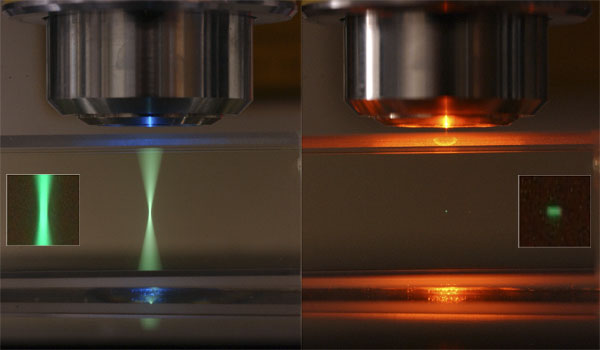
\includegraphics[width=4.5in]{1Pvs2PFluorescence.png}
\caption{A blue (488nm) laser of the sort used in confocal imaging excites an entire column of sample leading to green fluorescence (left).
A pulsed IR laser excites only at the focal point, as this is the only location where the density of photons is great enough for the 2-photon effect to take place.}
\label{1pvs2p}
\end{figure}

\subsection{Let's build a 2-photon!}
You have in front of you the transmission scanning microscope from before. 
\begin{itemize}
    \item What one thing do you need to change in order to excite a thin optical plane?
    \item Read the safety information on the next page. Modify your setup and use a green fluorescent slide to verify that it works. 
\end{itemize}


\clearpage
\section{IMPORTANT SAFETY INFORMATION}
Read this laser safety information before beginning. 
The following information should have been conveyed to you verbally. 
Please ask if you did not receive verbal instruction or if you have questions about laser safety. 

You will be working with a high energy pulsed laser capable of instantly blinding you should it enter your eye. 
During operation of the microscope the laser will be tuned to 920 nm which is invisible. 
Despite being invisible, the laser remains equally bright and equally dangerous.
Be very cautious around the set up:

\begin{itemize}
    \item Wear eye protection and use IR viewing cards as appropriate.
    \item Always be aware of the location of the beam and ensure everyone else in the room is also aware.
    \item Remove watches, jewelry, etc. Avoid directing the beam at shiny surfaces which could reflect it at unpredictable angles.
    \item Reduce laser power during alignment and tune the laser to visible wavelengths when possible.
    \item Shutter the beam when not using it. 
    \item Take particular care where the beam is directed upwards, such as in the periscope. 
    \item The scanners can deflect the beam by $>20$ degrees depending on the command signal. Ensure the mirrors are static and zeroed before routing the beam into the scan head for the first time. 
    \item Stand behind the scanners whilst the microscope is scanning.
    \item Use beam blocks where appropriate to keep the beam within your work area.
\end{itemize}

\clearpage

\section{Getting a basic 2-photon image}
 Figure~\ref{fig:layout} is a schematic of the beam path you have on the table. 
There is a shutter for safety, a beam expander to enlarge the beam so that it fills the scan mirrors, and a beam-splitter with a half-wave plate for altering laser power. 

At this point you have a functioning scan engine for a 2-photon.
Let's acquire an image! 
Your transmission-based scanning microscope used a photodiode and with the bright fluorescent slide your 2-photon can also do so.
However, as it stands the photodidoe will fail to provide you with an image?
Why is this and how do you need to modify it?
Perform the modification and use your scanning software to image the surface of the green slide. You should be able to see dust and scratches on the slide surface. 
\begin{figure}[h]
\center
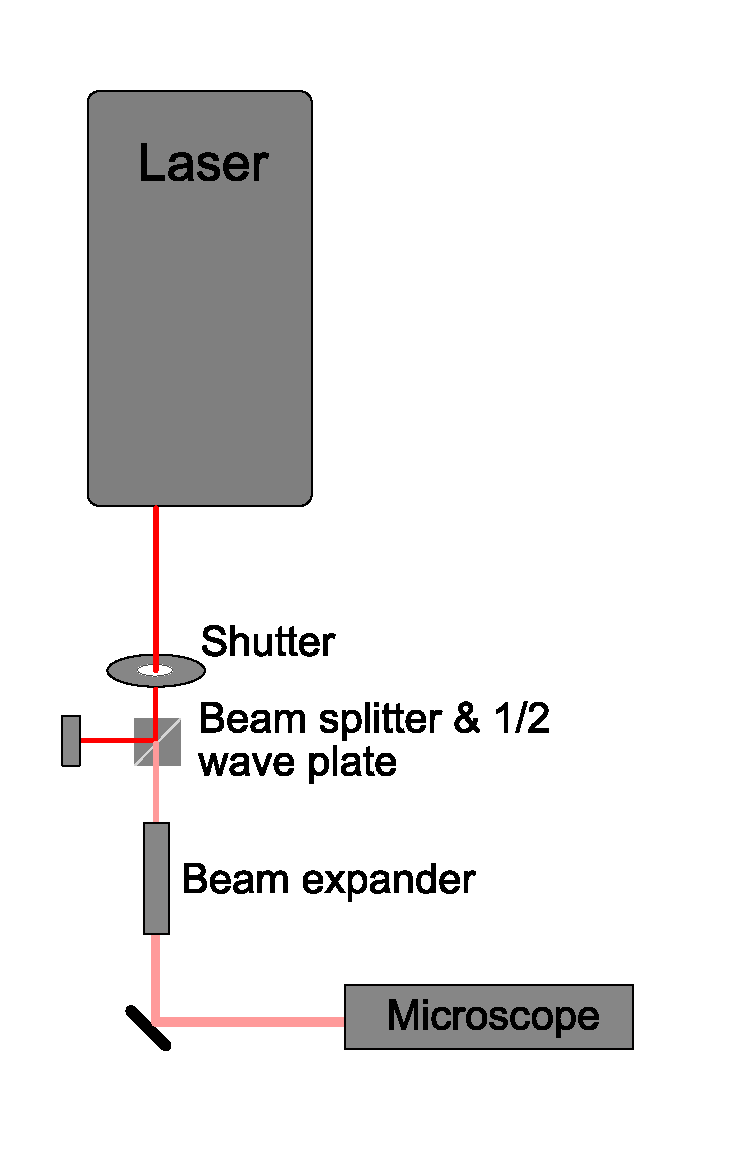
\includegraphics[width=3in]{2p_table_layout.eps}
\caption{Layout of the main light-path. Only key components are shown.}
\label{fig:layout}
\end{figure}

\clearpage

\section{Imaging pollen grains}
Pollen grains are the standard test sample of choice because they have micron-scale features and are brightly autofluorescent. 
Nonetheless, they are much dimmer than green fluorescent slide.
You will need assistance to replace the photodiode with a PMT.
The PMT is \textbf{delicate}. 
Do not expose it to even room light when powered on, as this will damage the photocathode. 
To increase the frame rate and obtain higher quality images you will switch from the prototype scanning software you have used until now to ScanImage, a MATLAB-based solution for 2-p imaging. 
Find pollen grains and obtain some images. 

\section{Making an upright microscope for imaging zebrafish larvae}
The 10x air objective you are using has an NA of about 0.2 whereas we usually perform 2-photon imaging using water immersion objectives with an NA of at least 0.8 .
How do you expect the image to change with a higher NA objective?

You will modify your microscope to convert it from a horizontal scan path to a vertical (upright) path that is compatible with a higher NA water immersion objective. 
This will allow you to obtain bright, higher resolution, images of pollen grains and then zebrafish larvae. 
Your microscope will look like that shown in Figure~\ref{fig:completed}.

\begin{figure}[h]
\center
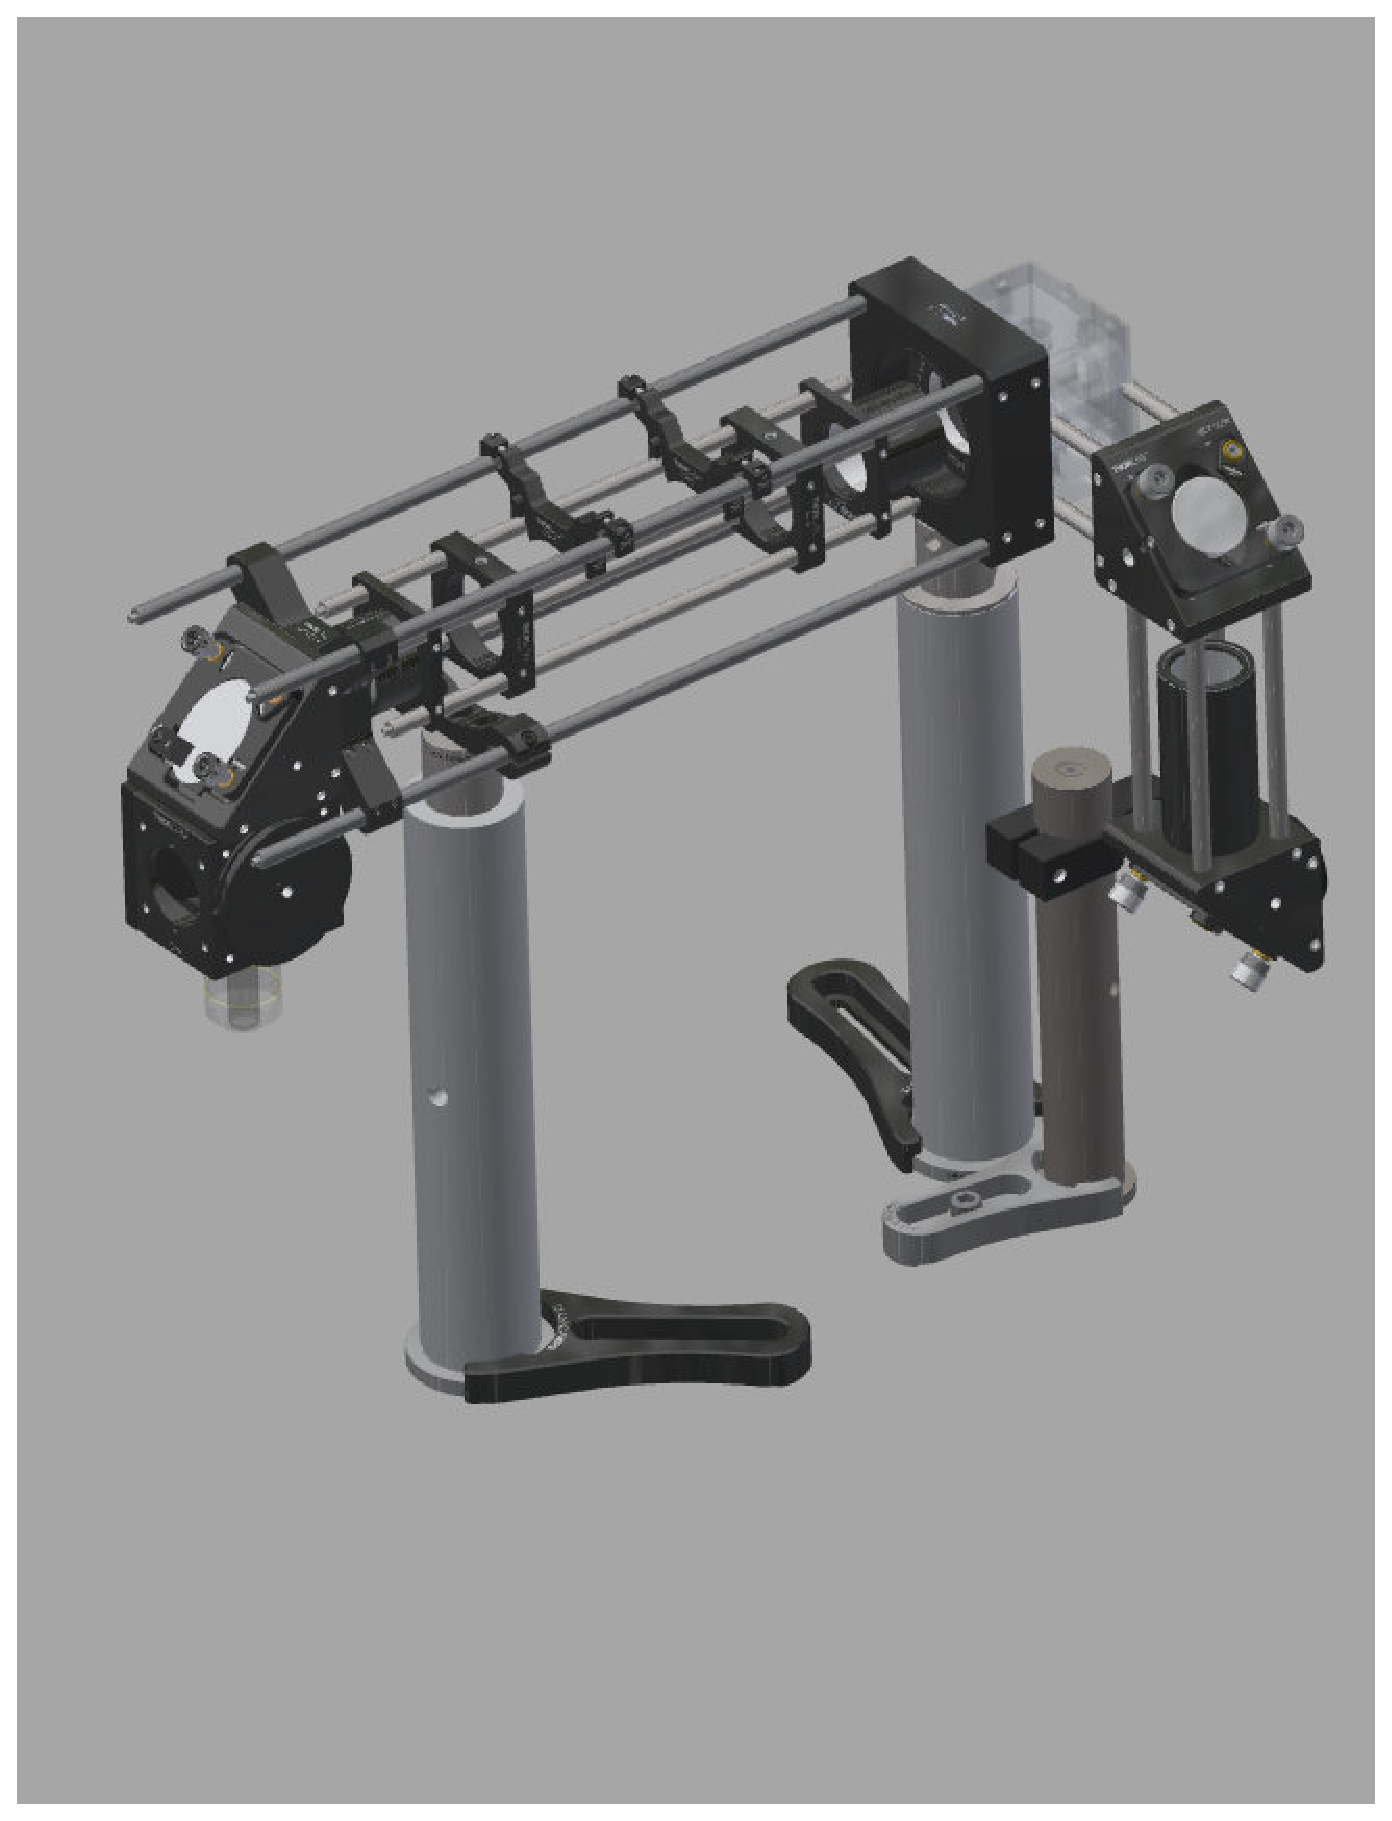
\includegraphics[width=2.0in]{./figures/completed_2p.eps}
\caption{Completed, upright, 2-photon minus emission path.}
\label{fig:completed}
\end{figure}

Remove the  objective and the end cage plate and replace with the dichgroic cube (Fig.~\ref{fig:dichroic_holder}.
Think before you do this, however. 
How far should the scanner relay optics be from the scanners and how far from the tube lens should the dichroic cube be mounted?
The path of the beam through the cube is depicted in Fig.~\ref{fig:dichroic_holder} as a red line.
To help you with this step, you can move the scanners over a small scan angle whilst looking at the the beam motion. 
Finally, is the beam exiting the cube traveling directly downwards and so on-axis with the objective we will add?

\begin{figure}[h]
\center
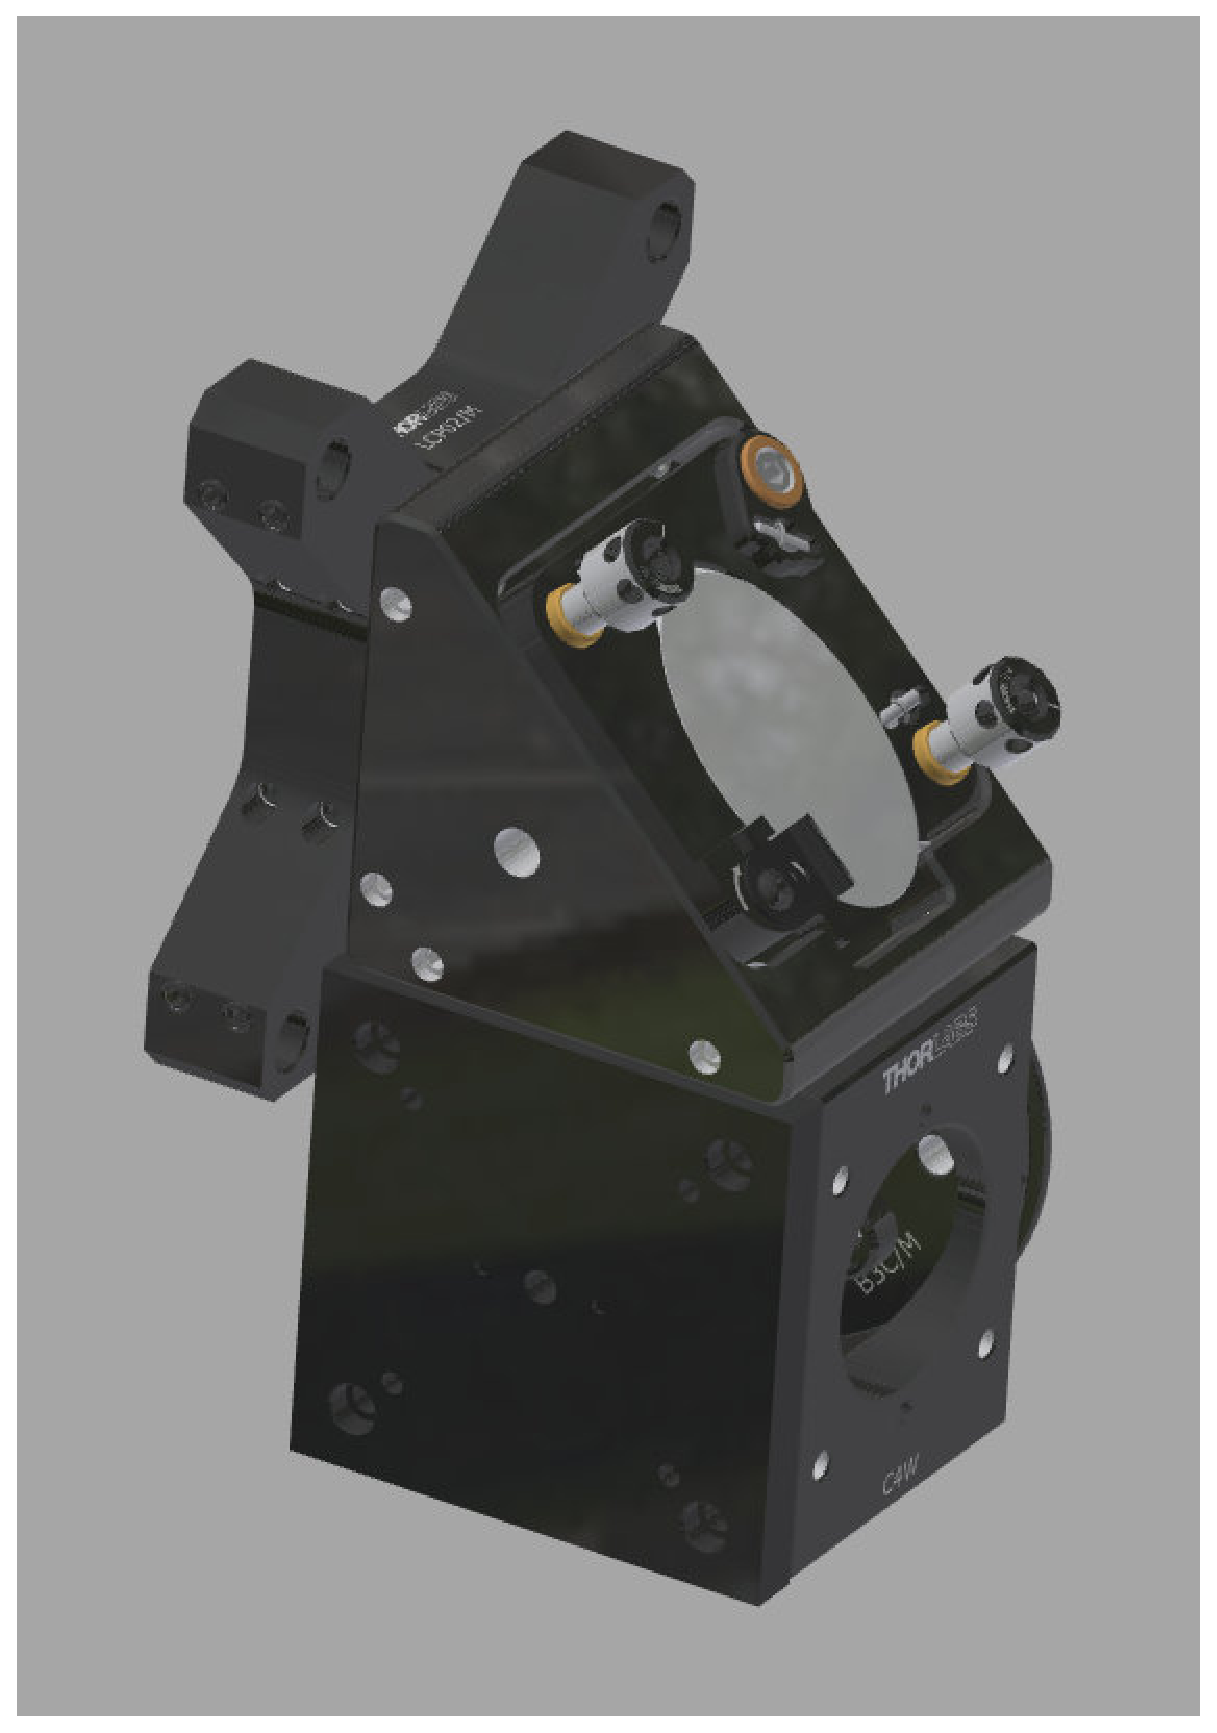
\includegraphics[width=2.0in]{dichroic_cube.eps}
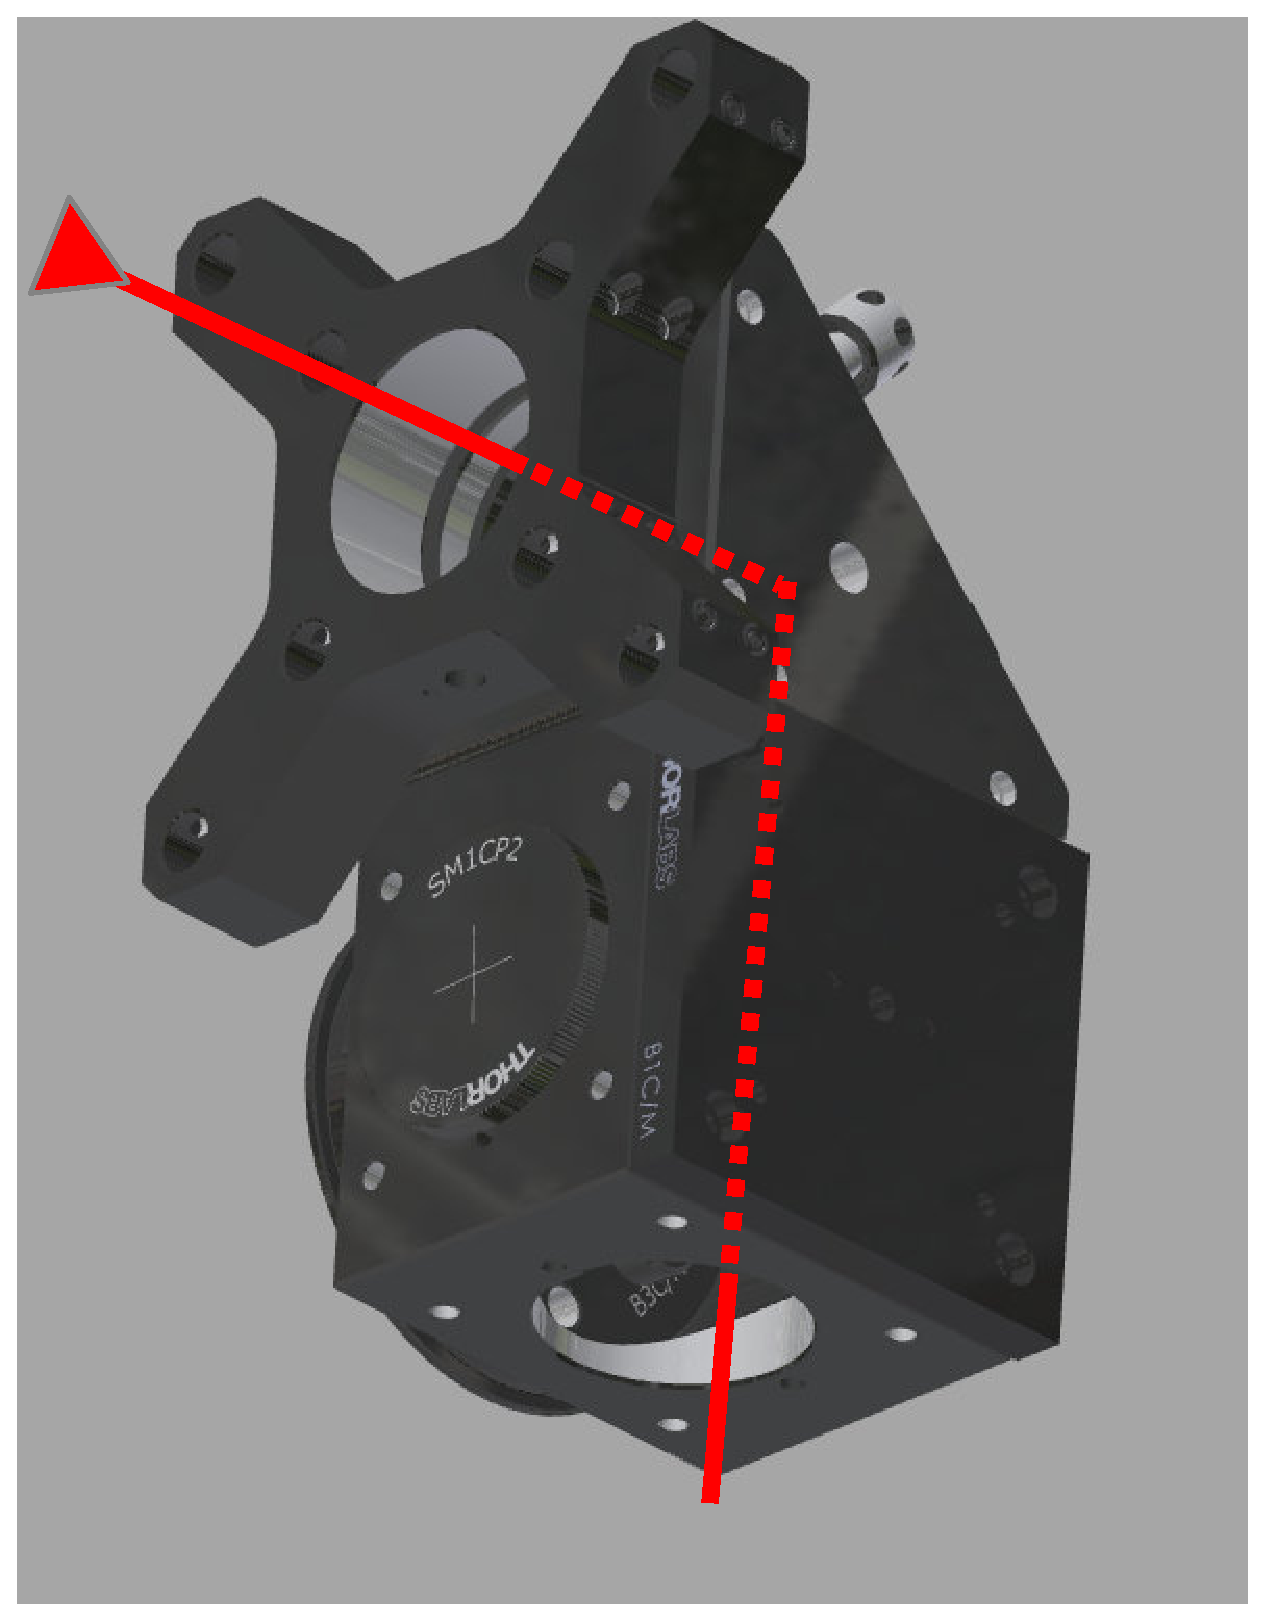
\includegraphics[width=2.0in]{laser_path_through_cube.eps}
\caption{Dichroic cube. Image on the right shows the path of the laser beam through the component.}
\label{fig:dichroic_holder}
\end{figure}

Once you are satisfied with the alignment, you can try scanning the fluorescent plastic sample card with the high NA objective. 

\subsubsection{Adding the emission path}
You now have a functioning excitation path but we still need to add the collection path. 
Instead of just dangling the PMT next to the sample, we will now use the objective to collect light (Fig.~\ref{fig:dichroic_holder_paths}). 
Think carefully what lens or lenses you need to add before the PMT. 
Hint: what should be conjugate with the PMT?
What other optical element do you need to add before the PMT?
Set this up and get good images of pollen grains. 
Once this is done you are ready for fish!

\begin{figure}[h]
\center
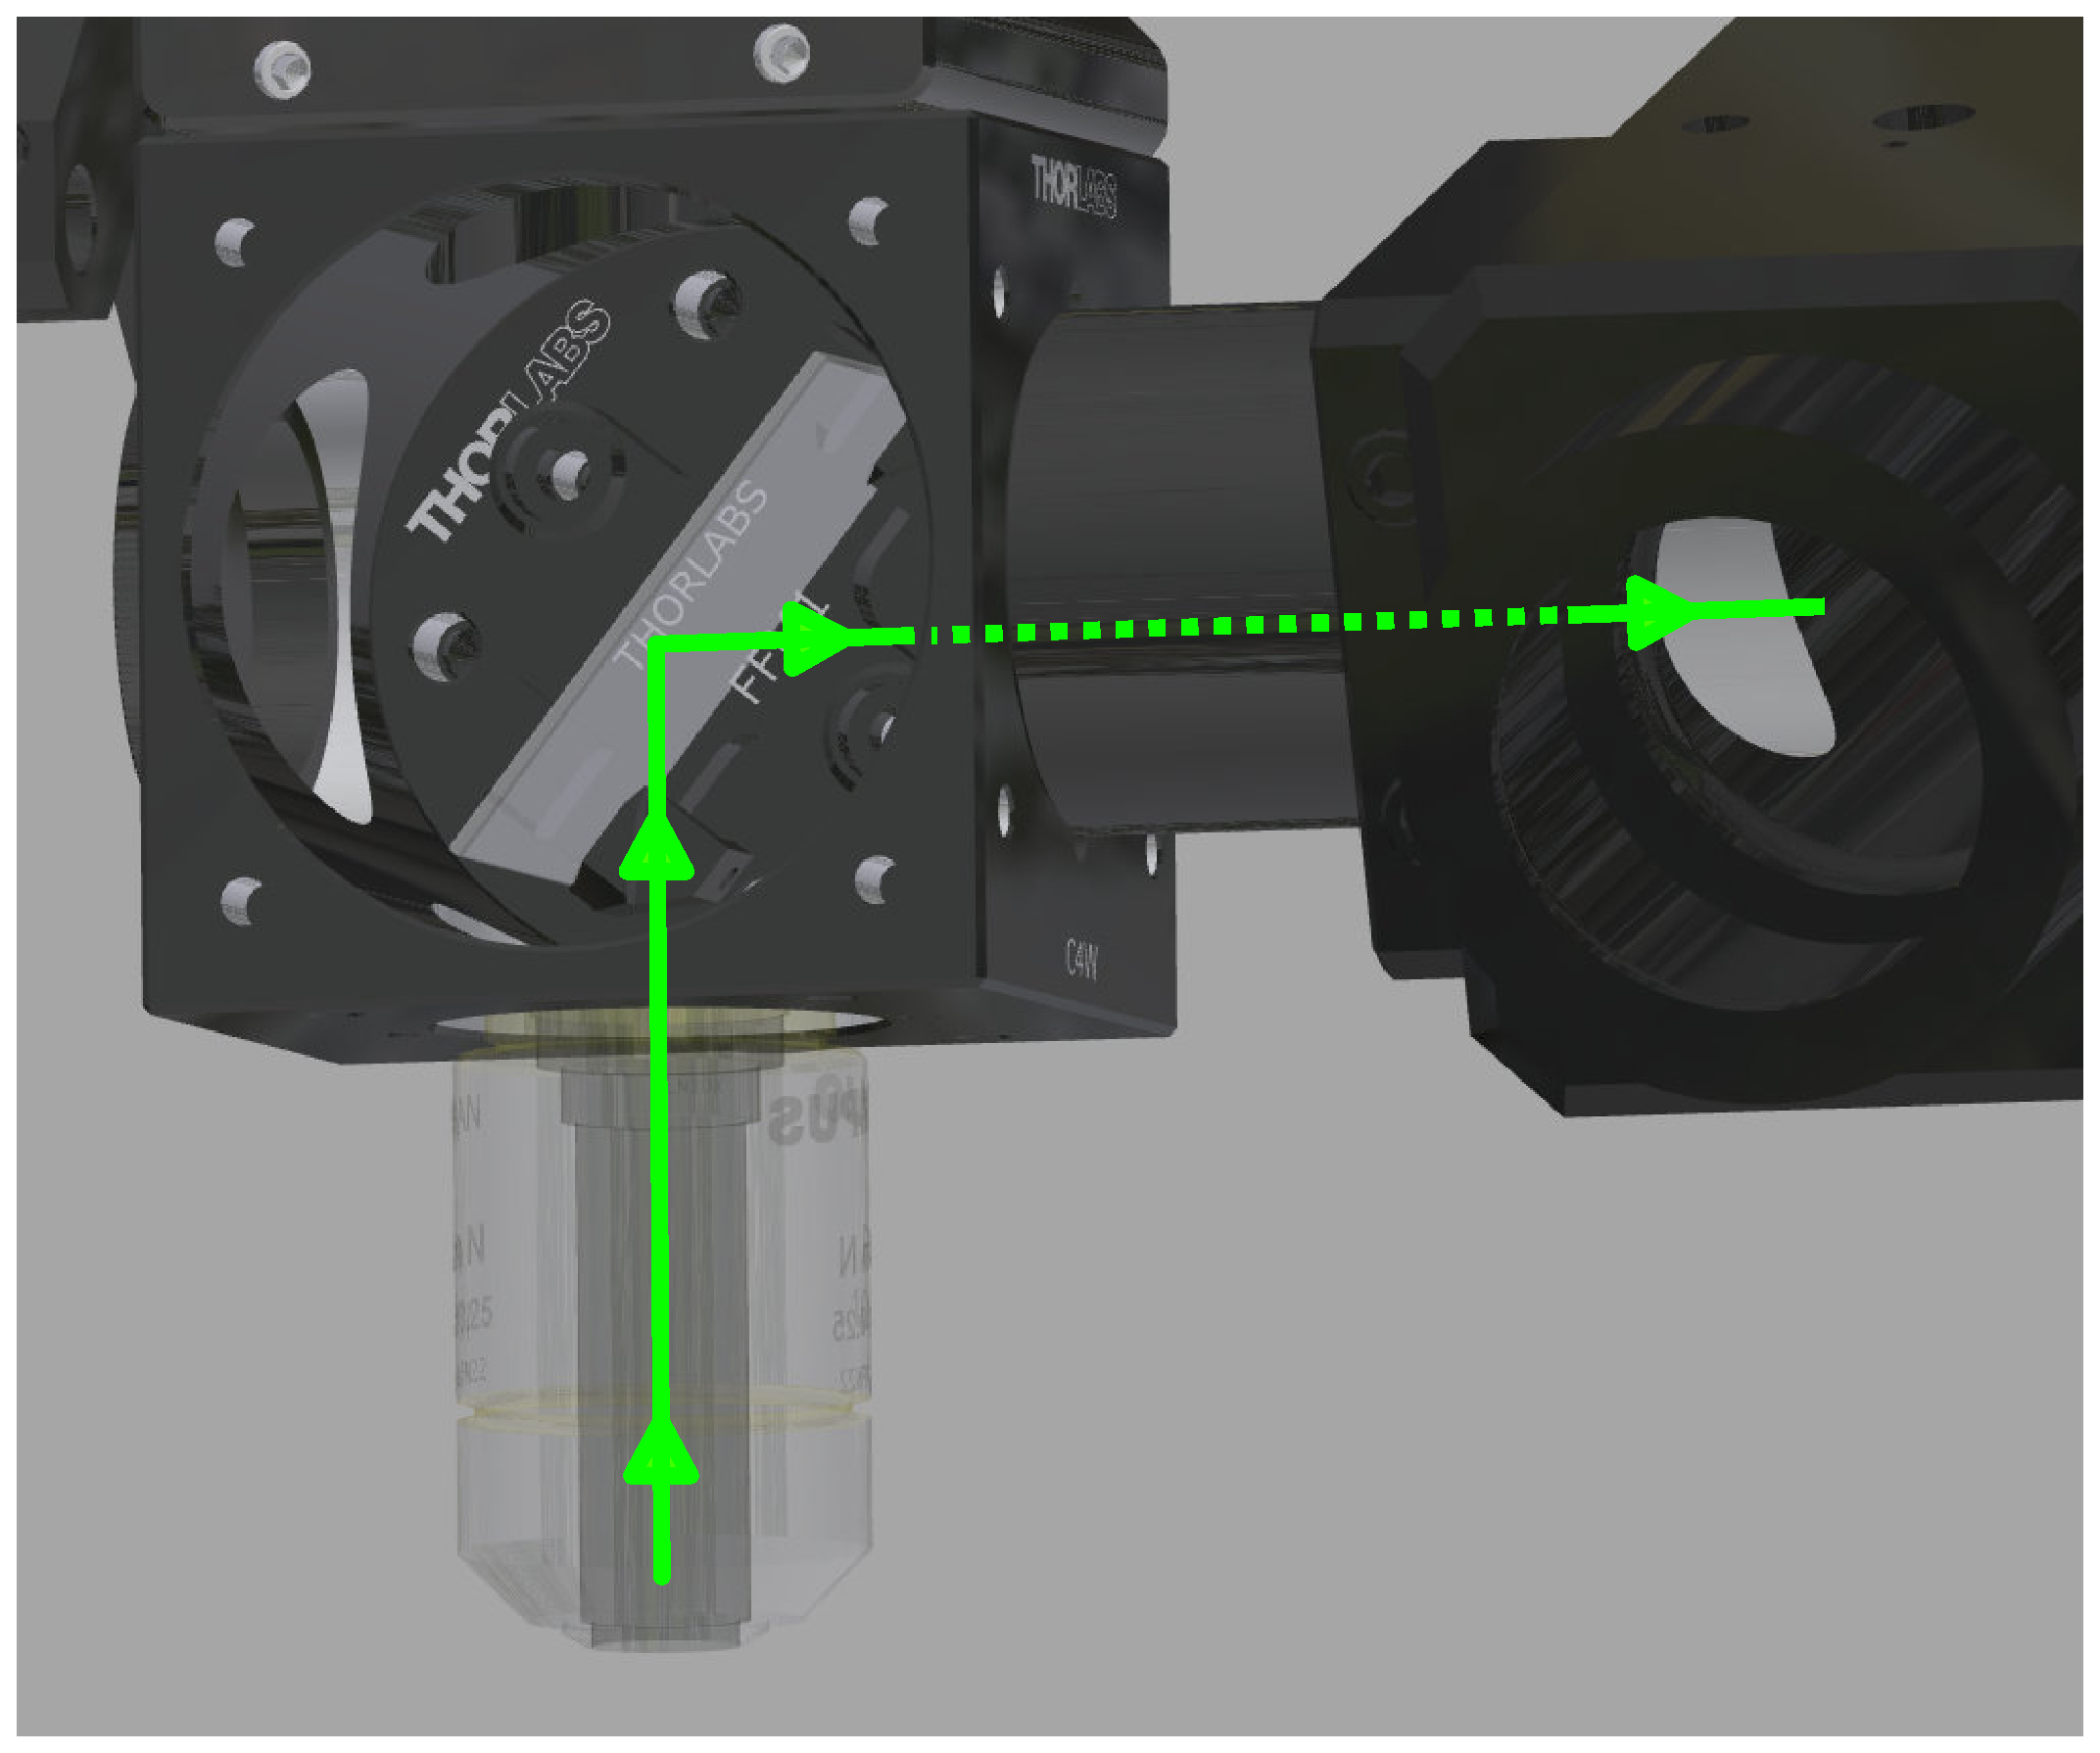
\includegraphics[width=3.1in]{cube_emission_cutout.eps}
\caption{Path of the emitted light through the dichroic cube. The cube's side-plate is removed to show the dichroic mirror itself. The illustration also shows the objective (transparent) and PMT holder (to the far right).}
\label{fig:dichroic_holder_paths}
\end{figure}




\end{document}